\documentclass{article}

% Language setting
% Replace `english' with e.g. `spanish' to change the document language
\usepackage[english]{babel}

% Set page size and margins
% Replace `letterpaper' with `a4paper' for UK/EU standard size
\usepackage[letterpaper,top=2cm,bottom=2cm,left=3cm,right=3cm,marginparwidth=1.75cm]{geometry}

% Useful packages
\usepackage{amsmath}
\usepackage{graphicx}
\usepackage[colorlinks=true, allcolors=blue]{hyperref}


\usepackage{listings}
\usepackage{color}

\definecolor{dkgreen}{rgb}{0,0.6,0}
\definecolor{gray}{rgb}{0.5,0.5,0.5}
\definecolor{mauve}{rgb}{0.58,0,0.82}

\lstset{frame=tb,
  language=bash,
  aboveskip=3mm,
  belowskip=3mm,
  showstringspaces=false,
  columns=flexible,
  basicstyle={\small\ttfamily},
  numbers=none,
  numberstyle=\tiny\color{gray},
  keywordstyle=\color{blue},
  commentstyle=\color{dkgreen},
  stringstyle=\color{mauve},
  breaklines=true,
  breakatwhitespace=true,
  tabsize=3
}


\title{Stock Tracking Application}
\author{LT1 - Jabagat, Jasmin, Roxas, Uy}

\begin{document}
\maketitle

\begin{abstract}
The Stock Tracking Application is a terminal-based application written in Python. It mainly uses the YFinance library for the backend and the Textual library for the terminal-based GUI. Users can look up stock information, create portfolios, and manage them. 
\end{abstract}

\section{Overview}

This documentation covers the installation, usage, and functionality of the application. 

\subsection{Features}

\begin{itemize}
    \item \textbf{Real-Time Stock Lookup} - The application can fetch the latest stock data using the \textbf{yfinance} python library. 
    \item \textbf{Terminal-Based GUI} - The application presents an interactive user interface that is built using the textual Python library. 
    \item \textbf{Track multiple stocks} - The application is able to track and save multiple stocks within a portfolio. 
    \item \textbf{Simulate a trading portfolio } - The application can track and simulate a trading portfolio by tracking its market value, simulate adding and selling positions, as well as calculating gains and losses based on based on the cost average of each stock in the portfolio.
    \item \textbf{Search of Tickers - }The application has a search function that facilitates the Buy Stock function.
\end{itemize}


\section{Manual and Documentation}

\subsection{Prerequisites}

Before installing the application, ensure you have installed Python 3.8 or later on your system. You will also need the following Python libraries:
\begin{itemize}
    \item \textbf{yfinance}: For fetching stock market data.
    \item \textbf{textual} - For creating the Terminal-Based GUI.
    \item \textbf{pandas}  - For operations in the application that require dataframes.
    \item \textbf{numpy} - For the required numerical computations on n dimensional arrays.
\end{itemize}
In order to lookup stock information and market prices, the application would also need internet connectivity. 


\subsection{Step-by-Step Installation}

\begin{enumerate}
    \item Clone the repository:
    \begin{lstlisting}
        git clone https://github.com/lsroxas/pds-lt1-stock-tracker
    \end{lstlisting}
    \item Create a Virtual Environment (Optional but Recommended)
    \begin{lstlisting}
        python3 -m venv venv
        source venv/bin/activate # On Windows use `venv\Scripts\activate`
    \end{lstlisting}
    \item Install Dependencies. Navigate to the application folder under the App folder:
    \begin{lstlisting}
        pip install -r requirements.txt
    \end{lstlisting}
    Alternatively, you can install the libraries individually:
    \begin{lstlisting}
        pip install yfinance textual pandas numpy
    \end{lstlisting}
    \item Run the Application
    \begin{lstlisting}
        python StockTrackerApp.py
    \end{lstlisting}
\end{enumerate}

\subsection{Navigating the Interface}

The main window \autoref{fig:1} of the application contains the following elements:
\begin{enumerate}
    \item \textbf{Portfolio Table}. This table contains the stocks already in your portfolio. It includes the latest market price, the average price at which all the same stocks were bought, and the gains/losses measures.
    \item \textbf{Portfolio Summary}. This contains data on when the portfolio's data was last refreshed and a summary of its value.
    \item \textbf{Main Action Buttons}. This contains buttons that simulate actions relating to stock trading for the portfolio. 
    \item \textbf{Application Footer}. This contains keyboard shortcuts for options available within the app. 
\end{enumerate}

\begin{figure}
    \centering
    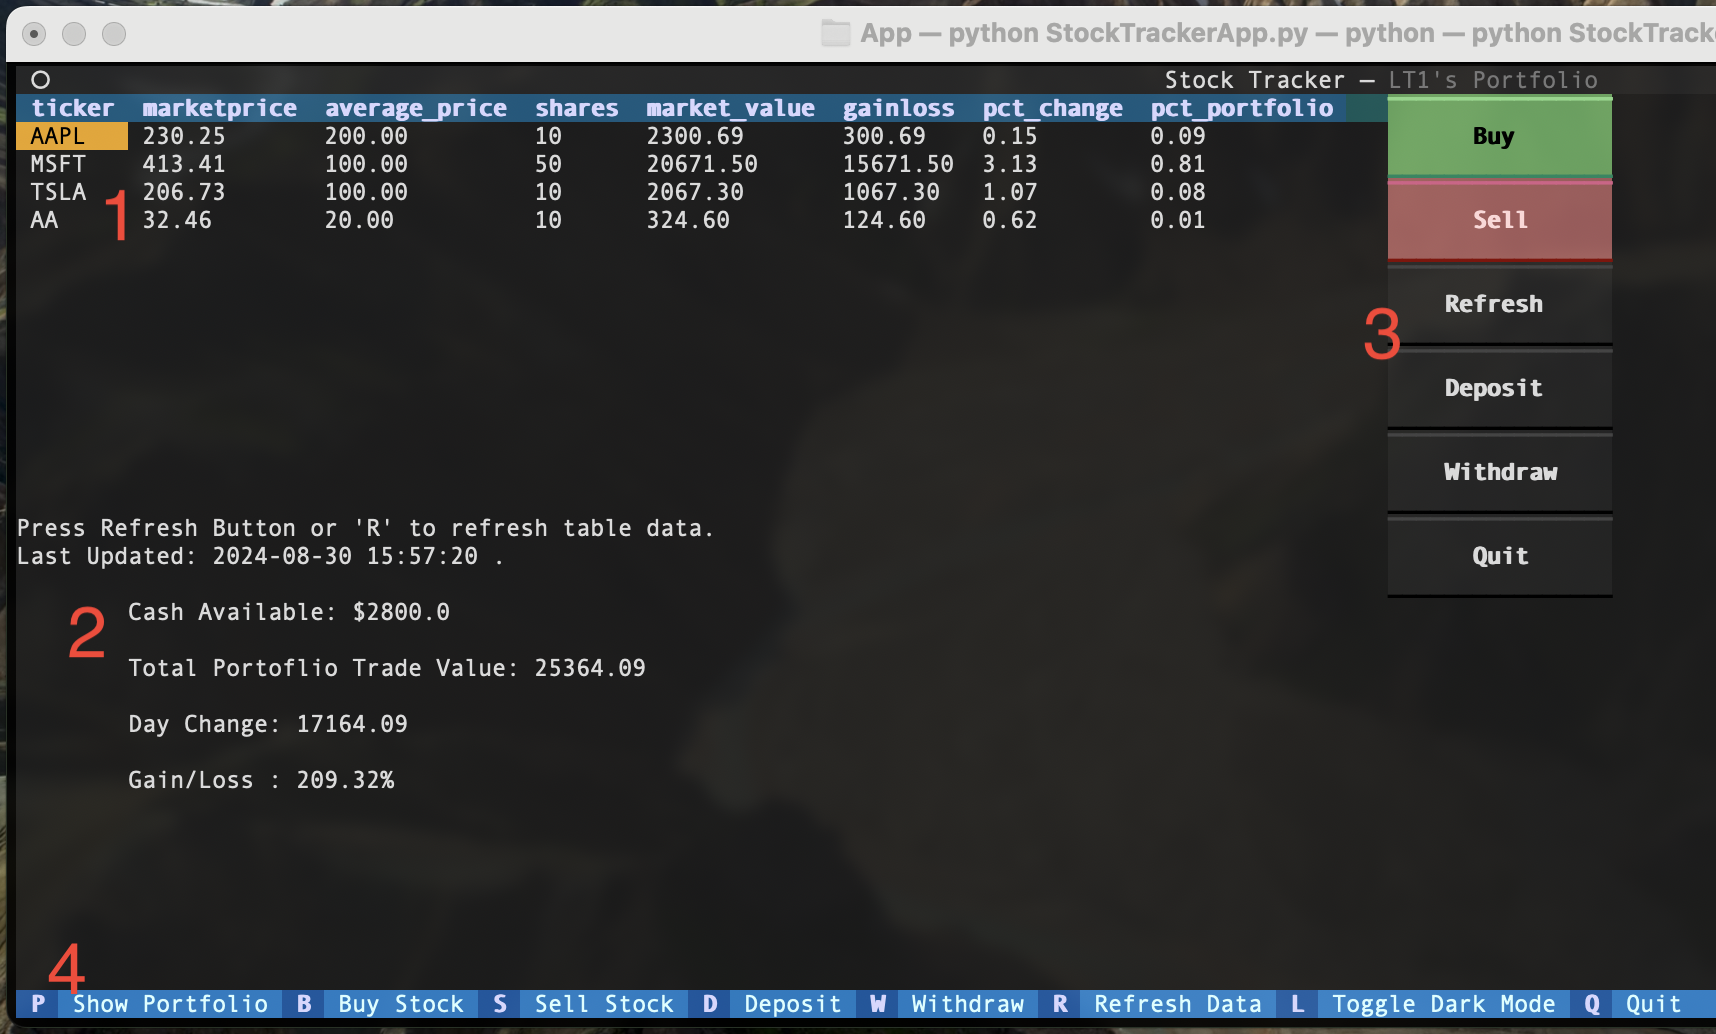
\includegraphics[width=1\linewidth]{MainWindow.png}
    \caption{Main Interface of the application}
    \label{fig:1}
\end{figure}

\subsection{Usage}

\subsubsection{Buying Stocks}

Clicking on the \textbf{Buy} button will bring up the Buy Stock screen \autoref{fig:2}. To simulate the action of buying stocks, you will need to:

\begin{enumerate}
    \item Search for the appropriate company ticker in the input text box. Note that company tickers are case-sensitive and are expected to be capitalized. 
    \item The application immediately begins searching Yahoo Finance for existing tickers equal to what is already typed in. The corresponding company name of the ticker would be reflected in this portion of the window. Tickers that are not valid would show blanks.
    \item Enter the sale price at which the stock would be bought. This input box accepts only numeric values. 
    \item Enter the amount of stocks that will be bought for the transaction. This input box accepts only integer values.
    \item Enter an amount for the transaction fee that will accompany the sale. This will be included in the total cost of the bought stocks and would affect the overall stock price average in the portfolio. This input box accepts only numeric values.
    \item Click on the \textbf{Execute} button to complete the transaction. You also have the option to cancel the sale and go back to the main window by clicking on the \textbf{Back to Portfolio} button.
\end{enumerate}

    Once the sale is done, a confirmation message will appear on the screen for successful transactions. A corresponding message will appear if there is an error \ref{fig:3}. 
    
    A transaction will not be successful if there is not enough money in the portfolio to cover the total cost of the stock purchase. 

    After completing all buy transactions, the user can click \textbf{Back to Portoflio} to return to the portfolio page. From there, the \textbf{Refresh} button needs to be clicked to update the displayed table.
 
\begin{figure}
    \centering
    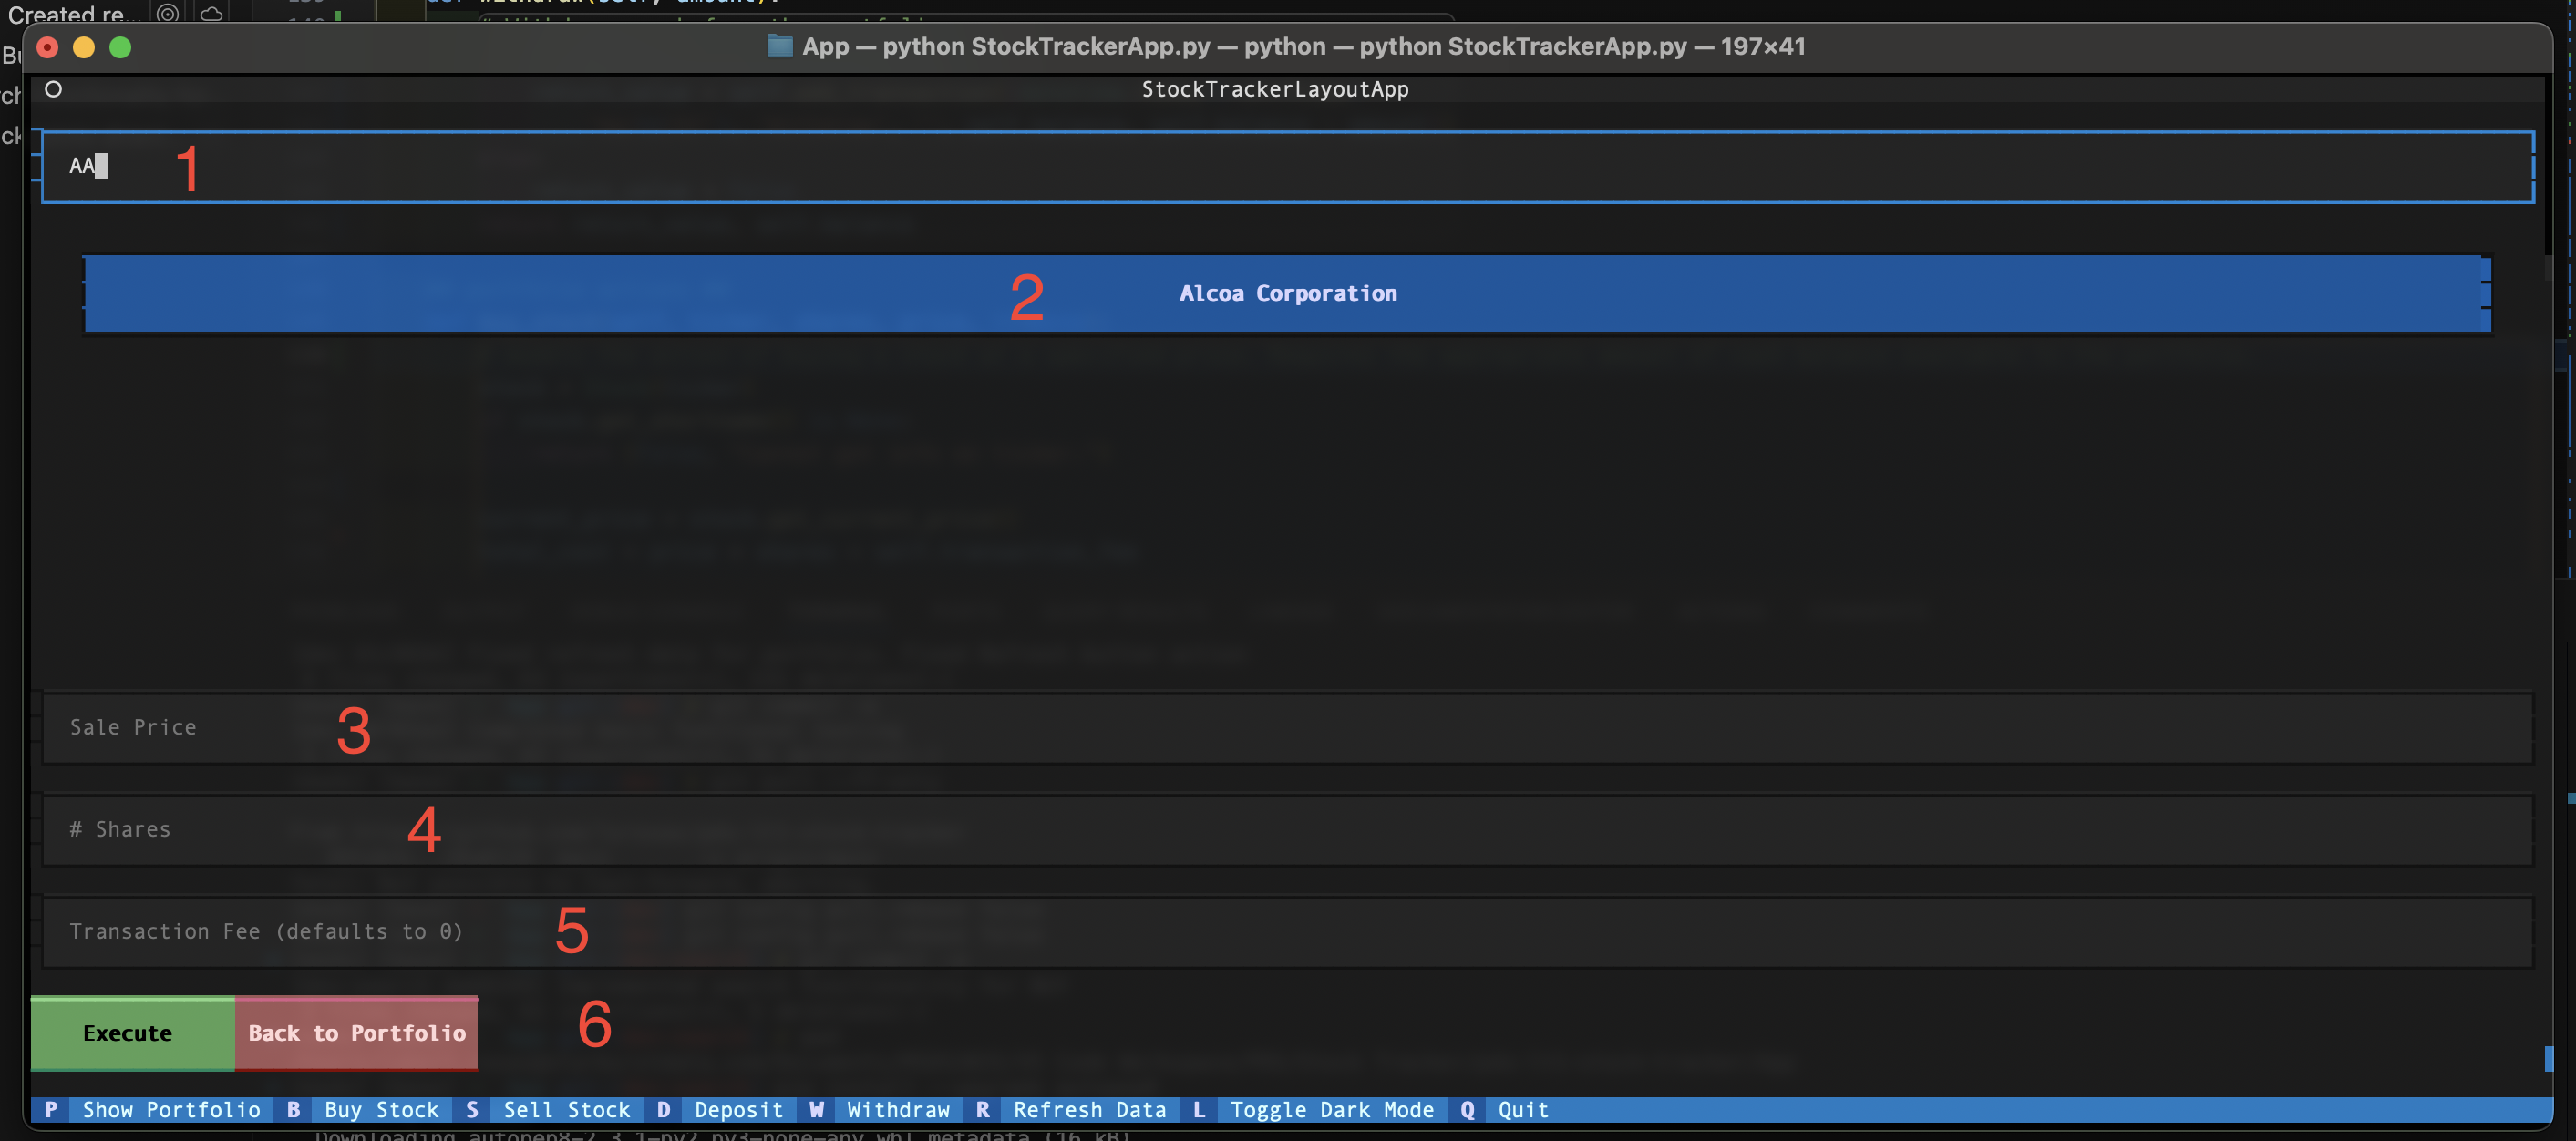
\includegraphics[width=1\linewidth]{BuyScreen.png}
    \caption{Buy Screen}
    \label{fig:2}
\end{figure}

\begin{figure}
    \centering
    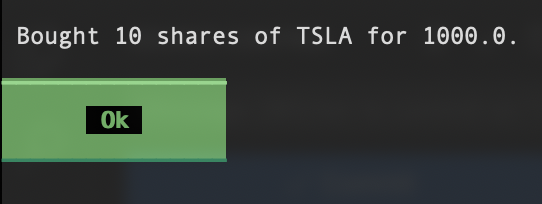
\includegraphics[width=1\linewidth]{BuyScreenConfirmation.png}
    \caption{Buy Screen  Confirmation}
    \label{fig:3}
\end{figure}


\subsubsection{Selling Stocks}

Clicking on the \textbf{Sell} button will bring up the Sell Stock screen \autoref{fig:4}. To simulate the action of selling stocks, you will need to:
\begin{enumerate}
    \item Enter the ticker of the stock you wish to sell. 
    \item Enter the desired selling price. This input accepts only numeric characters.
    \item Enter a number of shares to sell. This input only accepts integers. 
    \item Enter the corresponding Transaction Fee. This will be computed and added to the Portfolio cash. 
    \item Click the \textbf{Execute} to finalize the sale. Once successful, a message will pop up confirming the trade. \autoref{fig:5}
\end{enumerate}
    The revenue generated by the sale will be rolled to the portfolio's cash. If the ticker entered is not part of the portfolio, or if there aren't enough shares to cover the desired number of shares to sell, then the transaction will fail.
    
    After completing all sell transactions, the user can click \textbf{Back to Portoflio} to return to the portfolio page. From there, the \textbf{Refresh} button needs to be clicked to update the displayed table.

\begin{figure}
    \centering
    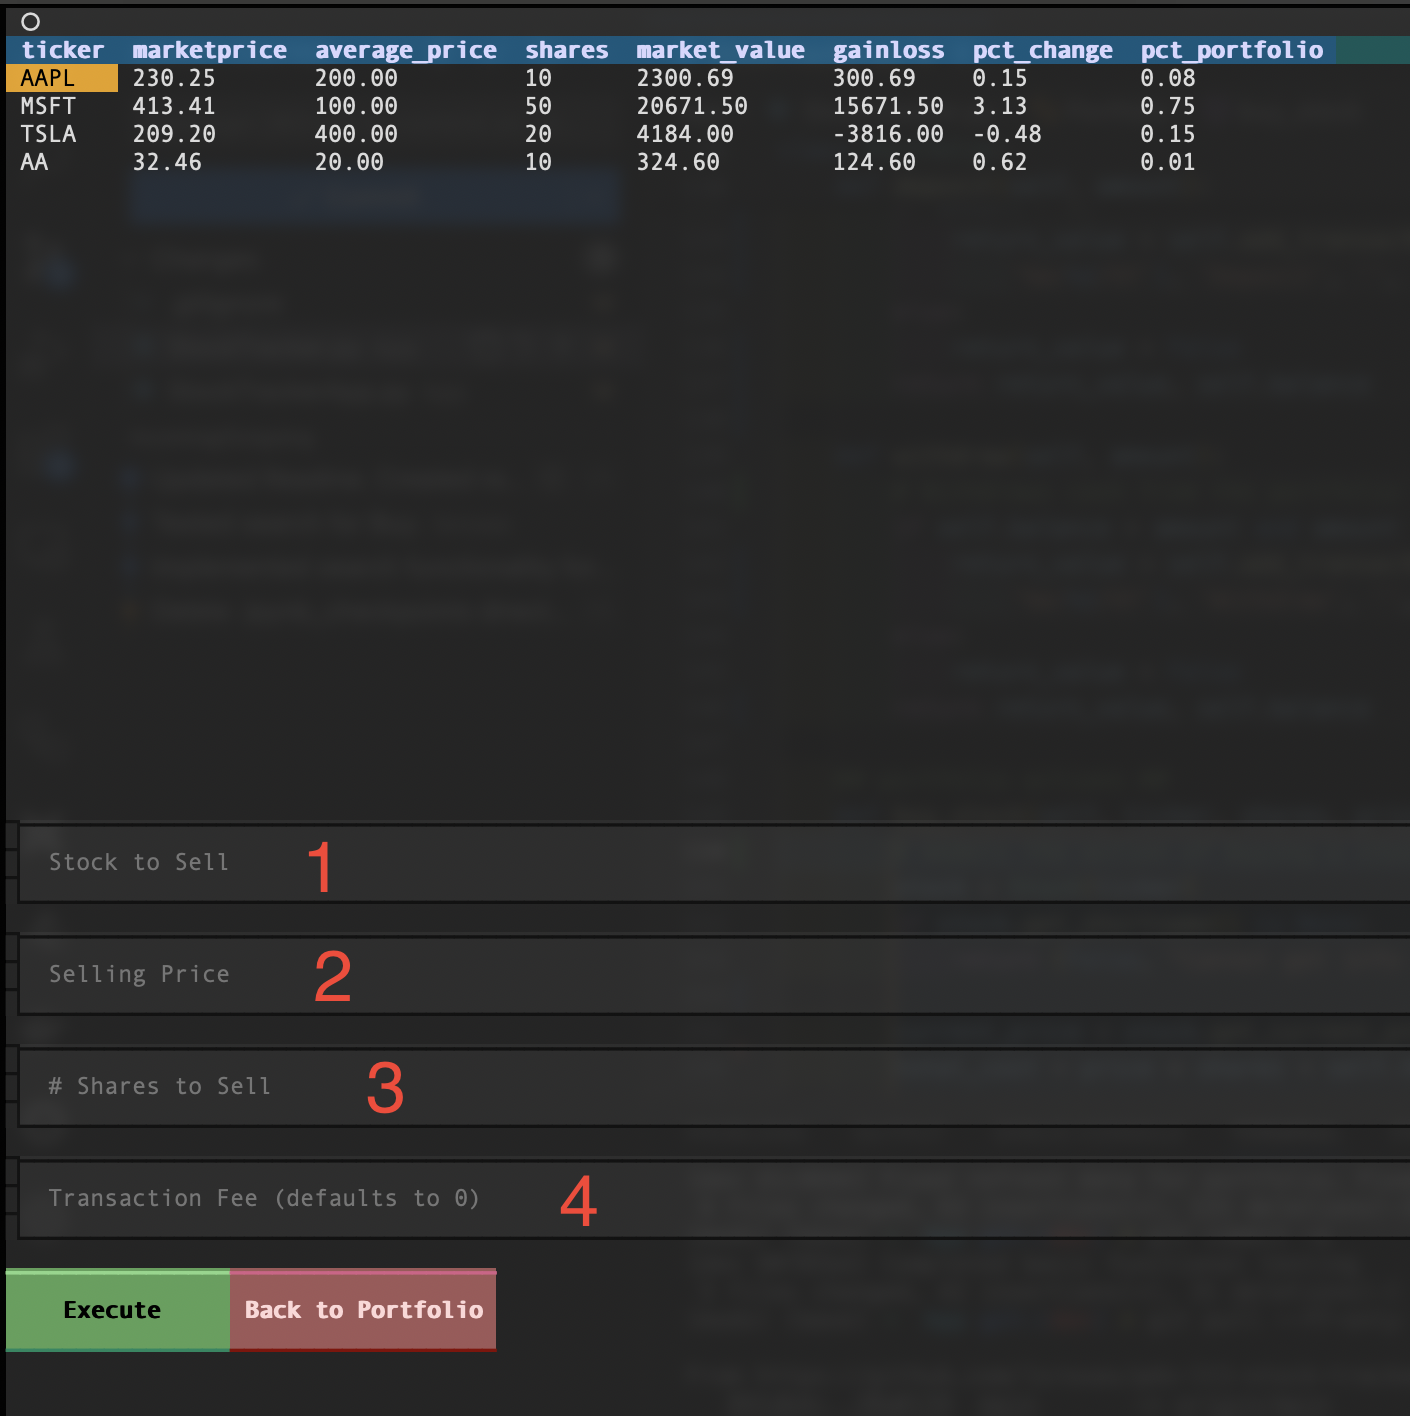
\includegraphics[width=1\linewidth]{SellScreen.png}
    \caption{Sell Screen}
    \label{fig:4}
\end{figure}

\begin{figure}
    \centering
    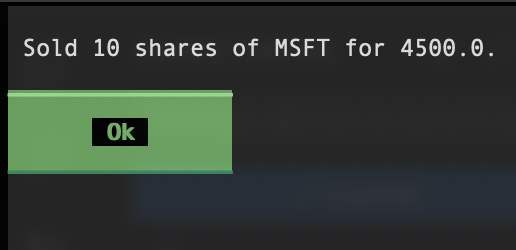
\includegraphics[width=1\linewidth]{SellScreenConfirmation.png}
    \caption{Sell Screen Confirmation}
    \label{fig:5}
\end{figure}

\subsubsection{Depositing and Withdrawing Money}
The application enables you to add or subtract money to and from the portfolio using the \textbf{Deposit} and \textbf{Withdraw} buttons. Both screens require you to enter an amount and confirm the action. \autoref{fig:6} \autoref{fig:7}Once confirmed, a message stating whether the transaction was completed successfully will appear. 

\begin{figure}
    \centering
    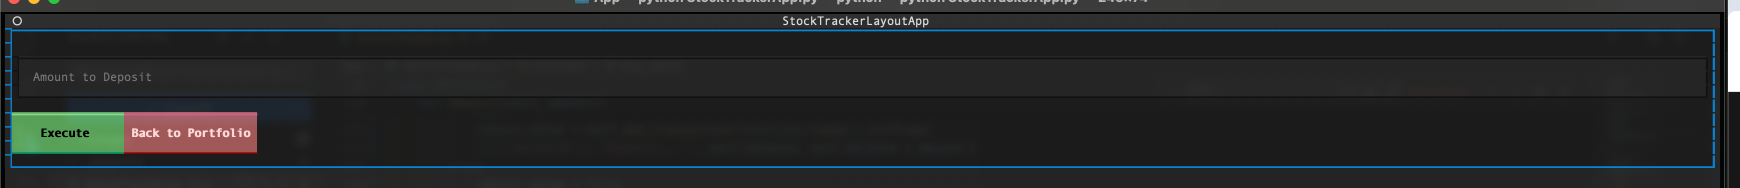
\includegraphics[width=1\linewidth]{Deposit.png}
    \caption{Deposit Screen}
    \label{fig:6}
\end{figure}

\begin{figure}
    \centering
    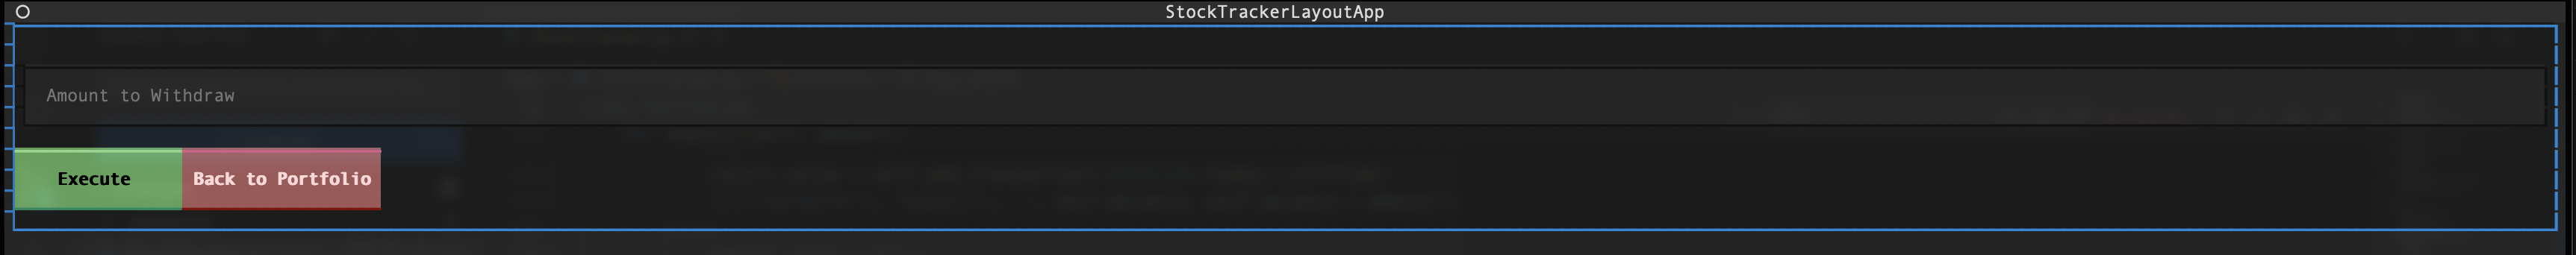
\includegraphics[width=1\linewidth]{Withdraw.png}
    \caption{Withdraw Screen}
    \label{fig:7}
\end{figure}

\section{Code Structure}

\subsection{StockTracker.py}
This file contains the main classes used by the application's backend. It includes 2 modules: The \textbf{Portfolio} and \textbf{Stock} classes.

\subsubsection{Stock}
This class contains methods and functions that interact with the \textbf{yfinance} library.
\begin{itemize}
    \item get{\_}shortname : Returns the company's short name from Yahoo Finance
    \item get{\_}info : Returns a dictionary containing information regarding the ticker symbol that was passed
    \item get{\_}name : Functions as a check whether a ticker is valid. 
    \item get{\_}history : Returns the stock price history of a given ticker
    \item get{{\_}}current_price : Returns the stock's latest price
    \item get{\_}ticker_current_price : The same as get_current_price but takes in a ticker for an input.
    \item get{{\_}}current{{\_}}prices : Returns the current prices for a list of tickers. 
\end{itemize}

\subsubsection{Portfolio}
This class contains methods and functions that handle the logic for the portfolio actions the application can do. A portfolio class is initialized with a starting balance (defaults to 10000), a default universal transaction fee (defaults to 0), and 2 csv files to store portfolio data and transaction data (defaults to portfolio.csv and transactions.csv respectively). 
\begin{itemize}
    \item load{\_}transaction:  Reads existing transactions from a csv file.
    \item save{\_}transaciton: Saves loaded transactions to a csv file.
    \item add{\_}tranction: Creates entris to the transactions dataframe. This includes buying and selling of stack, deposits, and withdrawals. 
    \item deposit: method that handles cash deposits to the portfolio.
    \item withdraw: method that handles the cash withdrawals from the portfolio.
    \item buy{\_}stock: method that handles the buy stock function of the application. 
    \item sell{\_}stock: method that handles the sell stock function of the application. 
    \item save{\_}portfolio: saves the portfolio dataframe to a csv file.
    \item load{\_}portfolio: reads portfolio data from a csv file and loads it to a dataframe.
    \item get{\_}portfolio{\_}value: calculates and returns metrics regarding the portfolio's values along with changes relating to changes in current stock prices.
    \item refresh{\_}data : gets fresh data from Yahoo Finance and loads it to the class. 
\end{itemize}

\subsection{StockTrackerApp.py}
This file is the application's main entry point. It defines and controls all the elements of the terminal-based GUI. The file follows the textual library's framework for deploying screens and widgets. The application has 5 screens:
\begin{enumerate}
    \item StockTrackerApp : Main display window. This contains the Portfolio display and action buttons. 
    \item BuyStockApp : Screen activated when buying stocks.
    \item SellStockApp : Screen activated when selling stocks. 
    \item DepositApp : Screen activated when depositing cash to the portfolio.
    \item WithdrawApp : Screen activated when depositing case to the portfolio. 
\end{enumerate}

The file also contains watchers for certain keystrokes that enable the application to render different screens based on keystroke information.

\subsection{Various .tcss files}
These files contain the formatting of the GUI elements and are used by the \textbf{textual} library to render applicable widgets. Entries are made in CSS format and are referenced by ids and class attributes in the GUI's widgets.



\section{References}

\begin{itemize}
    \item \href{https://pypi.org/project/yfinance/}{yfinance - PyPI page} - Official PyPI page for the yfinance library
    \item \href{https://textual.textualize.io/}{Textualize Official Documentation} - Documentation pages, tutorials and training for the textual library.
\end{itemize}




\end{document}

